\documentclass[12pt, letterpaper, titlepage]{article}

\usepackage{amsmath, amsfonts}
\usepackage{booktabs}
\usepackage{amsthm}
\usepackage{graphicx}
\usepackage[margin=1in]{geometry}
\usepackage{hyperref}
\usepackage{cleveref}
\hypersetup{colorlinks = true, linkcolor = blue, citecolor=blue, urlcolor = blue}
\usepackage{natbib}
\usepackage{float}
\usepackage{setspace}
\usepackage{pdfpages}
\usepackage[pagewise]{lineno}
\usepackage{mwe}
\usepackage{comment}
%\linenumbers*[1]
% %% patches to make lineno work better with amsmath
\newcommand*\patchAmsMathEnvironmentForLineno[1]{%
 \expandafter\let\csname old#1\expandafter\endcsname\csname #1\endcsname
 \expandafter\let\csname oldend#1\expandafter\endcsname\csname end#1\endcsname
 \renewenvironment{#1}%
 {\linenomath\csname old#1\endcsname}%
 {\csname oldend#1\endcsname\endlinenomath}}%
\newcommand*\patchBothAmsMathEnvironmentsForLineno[1]{%
 \patchAmsMathEnvironmentForLineno{#1}%
 \patchAmsMathEnvironmentForLineno{#1*}}%

\AtBeginDocument{%
 \patchBothAmsMathEnvironmentsForLineno{equation}%
 \patchBothAmsMathEnvironmentsForLineno{align}%
 \patchBothAmsMathEnvironmentsForLineno{flalign}%
 \patchBothAmsMathEnvironmentsForLineno{alignat}%
 \patchBothAmsMathEnvironmentsForLineno{gather}%
 \patchBothAmsMathEnvironmentsForLineno{multline}%
}

% control floats
\renewcommand\floatpagefraction{.9}
\renewcommand\topfraction{.9}
\renewcommand\bottomfraction{.9}
\renewcommand\textfraction{.1}
\setcounter{totalnumber}{50}
\setcounter{topnumber}{50}
\setcounter{bottomnumber}{50}

\newcommand{\jy}[1]{\textcolor{blue}{JY: #1}}
\newcommand{\eds}[1]{\textcolor{red}{EDS: (#1)}}


\title{Was Devon Allen Unjustly Disqualified at the 2022 World Track and Field Championships?} 

\author{Owen Fiore\\
%   \href{mailto:owen.fiore@uconn.edu}
% {\nolinkurl{owen.fiore@uconn.edu}}\\
  Elizabeth Schifano\\
  Jun Yan\\[1ex]
  Department of Statistics, University of Connecticut\\
}
\date{}

\begin{document}
\maketitle

%Abstract should be 200 words
%Devon Allen was disqualified in 2022... discussions about dq, talk methods and 
%models, venue effect, and conclusion
\begin{abstract}
  Devon Allen was disqualified in the Men's 110 meter hurdle final of the 2022
  Track and Field World Championships after registering a reaction time of 0.099 seconds, 0.001 
  seconds faster than what is allowed.  Following the games, bloggers on the running website 
  LetsRun scrutinized the results and performed non-statistical analysis of the data.
  They found that the reaction time data from the 2022 World Track Championships seemed to be faster 
  compared to the other datasets they looked at, but did not perform any meaningful statistical 
  analysis of the data.  This paper questions the reaction time disqualification barrier, which is
  currently 0.1 seconds to determine whether this is a reasonable threshold.
  We employ a generalized linear mixed model (GLMM) with a random effect term
  which will be referred to as the venue effect in order to try and model the
  data.  Additionally, we employ a signed-rank test for clustered data to compare
  reaction times for the same athletes at different competitions.
  This matter needs to be addressed because Devon Allen's disqualification could 
  be a problem that could continue to re-appear in future world championships.

  \jy{Avoid references in abstract.}

  
  \jy{This is only the background. An abstract also needs to summarize the contributions.}
%\bigskip
\noindent\sc{Keywords}:
Devon Allen, Reaction Time, Seiko, 2022 World Track and Field Championships 

\end{abstract}

\doublespace

\jy{The bib file needs quality control. The bib keys need to have a consistent
  style. I suggest using the keys from google scholar.}

\jy{Practice my writing tips in the stat-wriging notes: chapter 2 on
  latex. E.g., no vertical/horizontal lines in professional tables. Use the
  tables in my template.}

\jy{Turn on column numbers in your editor to keep line width under 80.}

\section{Introduction}
\label{sec:intro}


\jy{Not a good opening. Could start by telling the story, recapping the major
  events and discussions on the internet. Then dig into the relevant
  literature. Finally outline the contributions of this work.
}


\jy{use the following structure and flow:
  1) A paragraph to tell the story;
  2) A paragraph on informal statistical analyses on the internet/social media;
  3) A paragraph on scholarly articles on reaction time in the literature;
  4) A paragraph on what's new: methods; results.
  5) A paragraph of roadmap.}


1)
After coming in third in the 110 meter hurdles at the United States Track and 
Field Championships in Eugene Oregon at the end of June, Allen was expected to 
be a contender for the World Championships, which were scheduled for two months 
later, also in Eugene. At the World Championships, Allen made it through the 
heats and semifinals to reach the finals while posting reaction times of 0.123
in the heats and 0.101 in the semifinal.  Allen, who attended the University
of Oregon (Location of US World Championship and the World Championship) was
considered to be a favorite for the 110 meter hurdle after running 12.84 seconds
in early June; only 0.04 seconds away from the world record \citep{Preview}.
Thus his disqualification by reacting in 0.099 seconds instead of 0.01 was met
with shock from both Allen and fans alike.  NBC, who was broadcasting the
championships in the United States, later uploaded a video to their Youtube
channel that show the disqualification and can be found here:
\url{https://www.youtube.com/watch?v=D6NXTMo-1yM}. The crowd erupted with jeers when
they found out that Allen was disqualified, angry at the result.  Had Allen 
reacted just 0.001 seconds slower he would have been allowed to compete and been 
spared waiting another two years until the next World Track and Field Championship.

2)
Outside the blog posts from LetsRun.com, there have not been any published
papers regarding Devon Allen's disqualification in particular.  This is not
particularly surprising given that his disqualification occurred only last August.
Letsrun is a website that is part message board and part news.  The message board,
which functions similarly to Reddit is very active during important running
events, which include during the finals of major events such as
the Olympics and the World Track and Field Championships.  However, it is the
news section of the website that generated articles such as "Was Devon Allen
Screwed? There's At Least a 99\% That He Was" and "The Data Keeps Pouring In and
It Continues to Look Bad For World Athletics and Great For Devon Allen".  Robert
Johnson, who created and runs the Letsrun website argued that there was an error
with the timing equipment at the 2022 Track and Field World Championship and
cited graphs, statistics such as median reaction time, and compared the reaction
times at the 2022 Track and Field World Championship.  

3)
In 2009, the International Association of Athletics Federations (Also referred to
as IAAF or World Athletics), which is the governing board for international running
competitions, commissioned a study into changing the reaction time barrier.
The paper analyzed sprinters reaction times and the biological processes 
that went into reacting to the starting gun and concluded 
that athletes can react in as low as 0.08 seconds.  One study by Pain looked at
reaction times for nine male athletes and analyzed their reaction times.  The
fastest athlete of the nine, had on average (even with their two fastest time 
removed) a reaction time of 0.087 seconds and a standard deviation of 0.004
seconds.  Two other athletes were able to react similarly when under certain
muscular tightening conditions \citep{pain2007sprint}.
to IAAF that the disqualification barrier be decreased to allow sprinters to
react faster, and suggested 0.08 or 0.085 seconds as possible new thresholds.
Additionally, it was recommended to IAAF that high speed cameras be used to
change the reaction time criteria from pushing off on the block to body movement.
This could provide a more accurate representation of reaction time, and thus the
possibility of a false disqualification would be lowered \citep{komi2009iaaf}.  
A follow-up study from 2012 by Pilianidis, Mantzouranis, and Kasabalis found
significant differences between reaction times at several world championships
between 1997 and 2009 for the men's 110 meter hurdles.  Another important
conclusion was that for reaction times did not decrease over the twelve years
covered by the research in the study \citep{pilianidis2012start}.  This will
be important when considering the results in section \ref{sec:Results}.


Despite the study, IAAF has not changed the reaction barrier since it was
implemented at the 1999 World Track and Field Championships.  It is confusing
as to why IAAF would commission a study only to disregard the results and not
make the necessary changes.  It is unknown how many athletes since 2009 could
have potentially benefited from this, but it is probable that there are others
besides Allen who were disqualified.
%Reaction time barrier has been examined before: cite reviews
%Then go into specifics and talk about people who wanted to change barrier
%General reviews are important
%People have studied the biological processes, cite a few references
%How barrier is picked by regulator
%Read abstract and into and summarize into about one sentence what each paper contributes
%1 and 2 can be merged but 3 need to stand alone


4)
One of the first objectives of the paper is to try to model the data, which is
the reaction times of every non-disqualification since the 1999 World Championships. 
When determining the most effective model to use, several variations were
explored across the 4 different data sets: a linear model without a venue effect,
linear model with venue effect, a gamma model without a venue effect, a gamma model
with a venue effect, a gamma model without a venue effect and link set to log instead
of the default which is Gaussian.  The R package lme4 was very helpful with this
as it supported the Generalized Linear Mixed Model (GLMM) which allowed 
linear models with various distributions to be modeled\citep{Rpkg:lme4}.  The
model we use is a liner model with a fixed effect and random effect and follows
the gamma distribution. The fixed effect comes in the form of an intercept, and the
random effect will be called the venue effect and is reflective of how significant
the changes in the reaction time is for each venue, i.e. the venue effect is 
responsible for the variation between years. 

Another objective of this paper is to compare data for athletes who have competed
at additional competitions to see how their reaction times compare from previous
competitions to this one. First we can look at the reaction times of athletes who competed at the
World Track and Field Championship in both 2019 and 2022 and compare the times,
and secondly we can look at how athletes performed compared to how they did at
their national/qualifiers meet.  We would expect that athletes of this caliber,
who are world-class athletes, to not improve significantly from one year to the
next.  In order to reduce any chances of athletes improving reaction time, we
can also look at data from qualifying meets.  Almost every athlete had to qualify 
by proving they are elite at the national level, usually by coming in at least
fourth. Thus, data was compiled on athletes who competed
at the 2022 World Track and Field Championships on what these athletes also ran 
at their country's national championship. If there was any argument that athletes
have improved their reaction time from 2019 to 2022, it should now be considered
nearly null, as the national competitions took place between June and July 2022 
and the World Championships were in August.  Thus, it should be expected that 
elite athletes such as these will not get reasonably faster in such a short time
span. The equipment used to measure reaction time cannot be guaranteed to be
the same from national to international competition, but the time span between
meets has been reduced considerably.
%Simplify contribution to one paragraph: collect data and formal statistical
%analysis such as model used
%Move a lot of this to methods section
5)
The rest of this paper is as follows: Section~\ref{sec:Data} describes how data was
collected and begins to detail the GLMM model which is further developed in the
Section~\ref{sec:Methods}.  The signed-rank test analysis for the same athletes is
also included in the Section~\ref{sec:Methods}.  The Section~\ref{sec:Results}
section provides the probabilities from the methods section and the paper ends 
by questioning the reaction time barrier.

%Follow Anthony's work, explicit references as to what each section does

%Seiko section should go in the Results section.  From results it seems reasonable
%question the data and talk about Seiko






\section{Data} \label{sec:data}

\jy{Describe you data types; give details on sources; introduce notations for
  both types of data
  present exploratory plots.}

  \begin{equation}
    Y_{ij} = \beta_0 + \beta_1 X_{ij} + \gamma_i + \epsilon_{ij}
    \end{equation}
    
    where $Y_{ij}$ is the response variable for observation $j$ in year $i$, 
    $X_{ij}$ is the predictor variable for observation $j$ in year $i$, 
    $\beta_0$ is the intercept, $\beta_1$ is the coefficient for $X_{ij}$, 
    $\gamma_i$ is the random effect term for year $i$, and $\epsilon_{ij}$ 
    is the error term for observation $j$ in year $i$.

  %yij denotes ith years and j is observation in year
  %yij will have clustered i and we use random effect to account for this
  %When model is presented talk about how I modeled yij
  %Zij where player is i and cluster, group is year and j
  %Test hypothesis that reaction times are the same vs that they are not
Something that is extremely important to note in the Data is the inconsistency of World Athletics 
in terms of how they penalize false starts.  From 2007-2009, the IAAF (the former name for World 
Athletics, and the governing body for the World Track and Field Champions) instituted a rule change
that allowed one warning false start before a sprinter was disqualified \citep{False-Start}  This 
essentially gave sprinters a second chance and reduced the penalty for a false start.  There were 
18 male and 7 female false starts at the 2007 World Championships, 18 male and 7 female starts at 
the 2009 World Championships. Starting in 2011, the rule was scrapped, and the old policy which 
automatically disqualifies runners who false start was reinstituted.  The effect? At the 2011 World
Championship there were 6 male disqualifications and 4 female disqualifications \citep{False-Start}. 
By returning to the harsher policy and cracking down on false starts, World Athletics had reduced the
number of false starts by two thirds. This was desirable for World Athletics as false starts can 
make already long track meets more tedious, both for athletes and viewers watching the 
television broadcast.  Since 2011, IAAF has instituted the one false start rule
\citep{Pilianidis}.

Data was copied from the World Athletics website and pasted into an Excel
spreadsheet. The data covers the men's 110 meter hurdles and the women's 100
meter hurdles from 1999 to 2022.  The variable of prediction interest is reaction
time, and the predicting variables are year, stage of competition (heats, 
semifinal, final), total time, and gender.  The data can be found in the appendix:.  
Factors such as name, country, and identification number were
not considered important for the purposes of this research besides the times for
Devon Allen and the other United States athletes mentioned above.  The variable "Stage"
refers to whether the observation occurred during the "heats" (Preliminary round) which
is denoted by "H" in the data, "S" for "semifinals" (Of which there are either 2 or 3 
heats each year), and "F" for finals. The variable "Gender" has levels "M" and "F" 
which stand for "male" and "female" respectively.  The variable "Batch" takes a 
numerical value and every heat of every round from 1999 to 2022 was assigned it's
own number.  This was added because of suspected issues that reaction time may be
correlated with other runners reacting quickly (one runner reacting quickly may
result in other runners reacting quickly).  There is no statistical signficance to
how the batches were labeled, they were ordered chronologically by meet but
reverse chronologically by year (Batch 1 is a preliminary Heat of 2022 and Batch
111 corresponds to the 1999 finals). The data that looked at in the paper
is best visualized using a box plot. Figure~\ref{fig:DataBoxPlot}.  Included are
box plots of the reaction times of the men's semi finals and finals pooled
together and just the finals.
%Fix quotations
%Dont need the titles will add captions, use width =5, height = 3 in aspect ratio
\begin{figure}[h]
  \centering 
  \includegraphics[width=\textwidth,height=4in]{DataBoxPlot}
  \caption{Boxplot of semifinals and finals data}\label{fig:DataBoxPlot}
\end{figure}

\begin{figure}[h]
  \centering 
  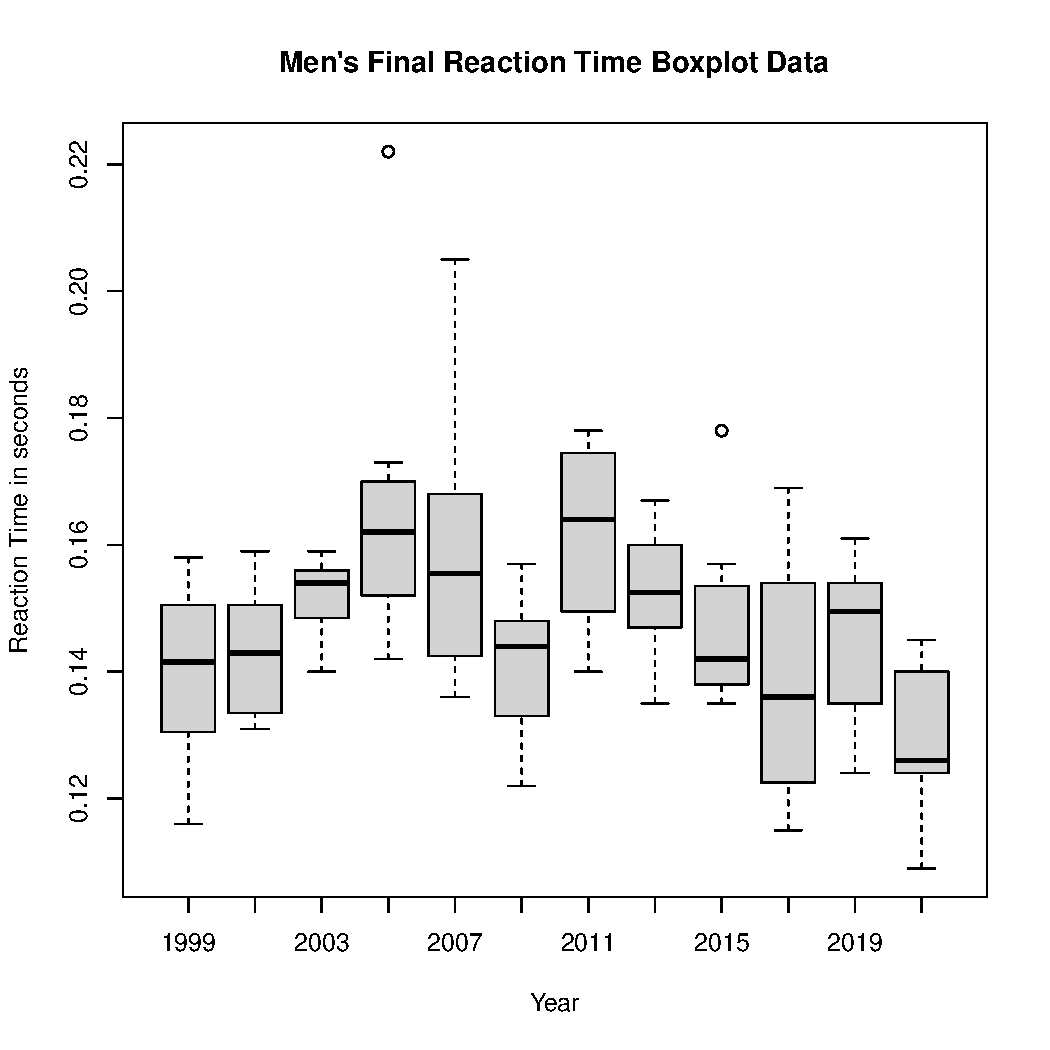
\includegraphics{BoxplotFinals}
  \label{fig:BoxplotFinals}
\end{figure}

This section was motivated from a qualitative analysis that started by looking
at how United States athletes reacted at the 2022 United States Track and Field
Championships. From June 23-26 2022, USA held its Track
and Field Championship to decide who to send to the World Championships at Hayward 
Field, the exact same venue as used for the World Track and Field Championship a month 
later.  Thus, a baseline is able to be established for the four USA athletes who 
competed in at least one round of both events: Trey Cunningham, Daniel Roberts, 
Grant Holloway, and Devon Allen. Every athlete reacted faster in all of the World 
Track and Field Championship races compared to the USA Track and Field 
Championship races. Devon Allen raced three times at the USA Track and
Field Championship and three times at the World Track and Field  Championship. 
His reaction times were significantly faster in the World Track and
Field Championship compared to the USA Track and Field Championship as were his
teamates.  This comparison suggests that the timing system used between the two
meets may have been meaningfully different to the point where Devon Allen was
disqualified more because of faulty equipment rather than because he reacted
too quickly.  This table below highlights the difference in reaction times for
Devon Allen, Trey Cunningham, Grant Holloway, and Daniel Roberts. "USA" denotes
the USA Track and Field Championships, "World" denotes the World Track and Field
Championships, "N/A" was used for any athlete that did not compete and thus
did not register a reaction time.  All numbers listed in the table are the reaction
time for the respective athletes in seconds. 


\begin{center}
  \begin{tabular}{|c c c c c c c|} 
   \hline
   Athlete & USA H & USA S & USA F & World H & World S & World F \\ [0.5ex] 
   \hline\hline
   Devon Allen & 0.201 & 0.153 & 0.160 & 0.123 & 0.101 & 0.099 \\ 
   \hline
   Trey Cunningham & 0.186 & 0.185 & 0.182 & 0.115 & 0.120 & 0.109 \\
   \hline
   Grant Holloway & 0.192 & 0.190 & N/A & 0.147 & 0.128 & 0.124 \\
   \hline
   Daniel Roberts & 0.181 & 0.200 & 0.183 & 0.179 & N/A & N/A \\ [0.5ex]
   \hline
  \end{tabular}
  \end{center}

This dataset is quite small to perform any formal statistical analysis on, but
the data was expanded to include data for athletes who competed at national
competitions (many of which were held from May-July of 2022).  Once the data
was collected, each athlete was designated to be a cluster and the stage of
competition (national or international) was specified to be the group. 

\section{Methods} \label{sec:meth}

\jy{set up the models/methods using the notations from last section; cite the
  right references.}

\subsection{GLMM}
%Include latex math symbols for the equations
A gamma mixed linear effects model was chosen as the best model to model the data.
Many models were tried and compared to determine what the strongest model.  For
a fixed data set such as the men's pooled data including 2022, the models with
the venue effect included performed better than the models without the venue
effect for each set of comparable models; as indicated by the lower AIC and
higher log likelihood.  Thus, the venue effect is significant and should be
included in the model.  It can also be established that a gamma distribution
better models the data than linear data from comparing the linear model with
venue effect and them gamma model with a venue effect.  The final decision that
was made in model selection was to include link = log in the model.  Despite
doing very little to alter the AIC or log likelihood, the log scale was included
in order to try and better deal with high outliers. %Include Residuals plot?

%Throughout exploratory analysis, gamma provides better AIC
%Spend paragraph on after fitting the model how to figure out 0.1 p value



Once the Gamma mixed effects model was chosen, it needed to be decided which combination
of effects to use.  It was possible to include a venue effect, a batch effect, or a year
and batch effect.  Density plots were created that simulated the probability of a mean
density less than 0.1, which is the current threshold for a reaction time
disqualification.  The density plots are shown below.  The batch effect is very
difficult to explain or interpret as it means that some heats of races were either
faster or slower and that everyone in the batch reacted similarly.  Although
it is possible that one athlete reacting faster could lead to others reacting
similarly, this does not make much practical sense as the difference between
heats that had fast and slow reaction times are all within 0.12 seconds of each
other.  It is much easier however to explain the venue effect.  The technology
that World Athletics has used has differed since 1999 and theoretically the
reaction time data from 2022 should be the best as the timing system should be
state of the art.  Any other weather or climate related factors such as humidity,
precipitation, elevation, etc. would all be negated when looking at the batch
effect, but are all factors that could potentially impact the venue effect.  


%T, generate from fitted model explain what
%The R code does.  Simulate from fitted model. Use distribution of model to 
%Figure out the p value of reaction time less than 0.1
To try and approximate the distribution of the reaction times, R code was written
to try and estimate the probabilities of observing a reaction time as extreme as
0.1 seconds.  The code re-paramertizes the gamma distribution to be in terms of
$\mu$ and shape rather than by $\alpha$ and $\beta$.

At a size of n=12,000,000, the calculated probability of a reaction
time being below 0.1 seconds was as follows for the various different data sets:

\begin{center}
  \begin{tabular}{|c c|} 
   \hline
   Data Set & Probability RxnTime < 0.1 \\ 
   \hline\hline
   all finals gamma log & 0.000864 \\ 
   \hline
   old finals gamma log & 0.000429 \\
   \hline
   all pooled gamma log & 0.006847 \\
   \hline
   old pooled gamma log & 0.005749 \\
  \end{tabular}
  \end{center}




\subsection{Rank-based comparison for Clustered}


%Citations needed
%Include math formulas and the test statistic
%Equation of test statistic is from papers cited by clusrank. Asymptootic dist
%Was found by __ referecne and the implementation is from the clusrank R package


The test statistic of the DS method of the Wilcoxon rank-sum statistic is:
$Z = \frac{S - E(S)}{\sqrt{\hat{\text{Var}}(S)}}$ where 
$W^* = \frac{1}{N} + \sum_{i=1}^{N} \delta_{i}^{*} R_{i}^{*}$, $R_{i}^{*}$ is
the rank of $X_{i}^{*}$.
The asymptomatic distribution of the Wilcoxon rank-sum statistic was found by
\citet{datta2005rank} and the R package "clusrank" allows for its implementation.
\citep{jiang2017wilcoxon}.


Using the "clusWilcox.test" function, a grouped and clustered Wilcoxon rank sum
test was performed with the cluster set to be the Athlete and group set to Year.
The method was set to be "DS" which is used for the Data and Satten method, which
is preferable when the cluster sizes are informative \citep{jiang2017wilcoxon}.  We do not care that some
athletes made it further in either competition than another or that it should
not matter how elite an athlete is at the 110 meter hurdles once we get to the
national international competition level.  Cluster sizes vary from 2 observations
to 6.

When the clusrank rank sum test was performed, the "ds" method produced a z score of
2.9751 and p value of 0.001464.  This value is for a one-sided test and show that
the mean reaction time on average in 2019 was larger than the mean reaction time
in 2022 for athletes who competed in both championships at an alpha level of 0.01.
This provides good evidence that athletes who competed in both 2019 and 2022 got
faster during that timespan.


Repeating the data collection steps and
again performing a clustered analysis for a Wilcoxon ranked sum test
results in two new z scores and p values.  The "ds" method produced a z score of
3.6069 and p value of 0.000155.  This result is highly significant and shows that
the times at the national stage of competition were significantly higher than
the reaction times at the World Championships even for an alpha level of 0.001.


\section{Results}
\jy{summarize your findings; discuss limitations and possible future works.}

%Table should go to the results section
All Men's semi finals and finals data
\begin{center}
  \begin{tabular}{|c  c  c  c  c  c  c |}
   \hline 
   Model & AIC & Log Likelihood & Int effect est & Int se & Int var & Resid Var \\ [0.5ex] 
   \hline\hline
   linear one & -1667 & 835.5 & 0.1529 & 0.0014 & N/A & N/A \\
   \hline
   linear year & -1713 & 859.3 & 0.1541 & 0.0040 & 1.719e-04 & 5.926e-04 \\ 
   \hline
   gamma one & -1756 & 880.2 & 6.554 & 0.0598 & N/A & N/A \\
   \hline
   gamma year & -1848 & 926.9 & 6.553 & 0.2269 & 0.1305 & 0.0234 \\
   \hline
   gamma one log & -1756 & 880.2 & -1.880 & 0.0091 & N/A & N/A \\
   \hline
   gamma year log & -1848 & 927.0 & -1.869 & 0.0348 & 0.0031 & 0.0235 \\ [0.5ex]
   \hline
  \end{tabular}
  \end{center}
%Section 4.1: Gamma model results show the fitting with and without 2022,
%talk about p values and thresholds from the simulations (do not include the
%results in the methods section). 
Using the gamma function with link set to log (whose summary statistics can be
found in the last row of the above table), the probability of the function being
less than 0.1 seconds can be calculated to see if Allen's disqualification was an anomaly.
Prior to the 2022 World Championship, there was a 0.0425\% chance (based on the
simulated results) of observing a reaction time below 0.01 seconds in the men's
finals.  That means that we would expect a time below the threshold to occur
once every 2,352 starts.  Considering there are roughly 8 men's finals reaction
times every 2 years (The World Championship is biennial), every 588 years there
should be a time as extreme as Allen's.  This seems extremely unlikely, and thus
it seems like there may be an additional explanation for the fast reaction times.

It is interesting that the probability of observing a reaction time below 0.1
seconds increases drastically for the finals data and increases by a smaller margin
for the pooled data set after 2022 is included in the data set.  By including 2022
in the data, the chances of observing an extreme time are increased, showing that
2022 is a high outlier for reaction times compared to other years.

It is worth noting that changing the reaction time barrier from 0.1 seconds to
0.08 seconds drastically reduces the chances of observing a reaction time that
would break the barrier.  For the dataset of all finals data, the probability
associated with observing a reaction time below 0.08 seconds was $6.67\cdot10{-7}$.
If IAAF were to change the reaction time the way that \citet{Komi}'s paper
suggests, the probability would be so much lower that athletes would likely not
have a case to make when arguing against a disqualification.

%Discussion should show that random effect
%and standard error increase and that 2022 is special.  Now talk about Seiko
%timing equipment

%Citation needed in this section
Since 1985 Seiko Holding Corporations has served every World Athletics Championship
as the official timer \citep{Seiko}.  Since 1985, the technology and the ability
to accurately predict measurements: long jump distances, false starts, total time,
reaction time, etc. have all dramatically improved.  Seiko did not start tracking
reaction time as an official measurement until 1999 in the men's and women's 100 meter
hurdles.  Seiko regularly updates their equipment so that they provide cutting edge
technology to the World Track and Field Championships, the highest stakes in the world
of running outside of the Olympics. Seiko's technology for detecting reaction 
times relies on the pressure that athletes
exert on the plate when they push off.  Their systems measure the time differential
between when the "gun" goes off to start the race and when the pressure changes 
\citep{Seiko}  If an athlete has a reaction time under 0.10 seconds, it is deemed a 
false start as it is considered that no athlete can react so quickly 
\citep{Seiko-Timing}.  Thus, a reaction time of for example 0.05, suggests that 
the athlete predicted the gun and it was luck that caused their abnormally high 
time.  At the World Championship level, World Athletics and Seiko want to remove 
that element of luck and thus impose the 0.1 second barrier. In 2013, Seiko 
upgraded their timing equipment for sprinting events (100 meter hurdles falls 
under this category) \citep{WorldAthletics_2013}.  Since 1999, the highest reaction 
times in the men's 110-meter hurdle were recorded in 2013.  That is not to say that the higher 
times were caused by Seiko's equipment, but the two may be related.  It is worth noting that prior
to 2022, Seiko again upgraded its technology but for its jump management system.



%Section 4.2 is motivated by seiko timing and look at same athletes across
%multiple types of competition: 2019 and national

%Discussion/Conclusion is beyond results.  Limitations, what type of data we
%hope to have.

For the comparison between athletes who competed in 2019 and 2022, the p value
was 0.001464.  As Seiko timed both events, there should not be a signficant
difference if the timing equipment in both instances was working correctly.
Additionally, the p value was 0.000155 for the same athletes competing in the 
same year  To put it simply, there is not a reasonable explanation for 
this. It is inconceivable that so many athletes would improve such a significant
amount in such a small amount of time. 6 countries are represented in this 
comparison, which drastically decreases the chances of this issue being caused by
one specific country.  The United States athlete's improvement in times was
discussed earlier in the paper, but this data shows that on average there was
%Use a reference in this part
improvement for British, Polish, French, Brazilian, and Spanish athletes.


%Wrap up and Conclusion
It is worth noting that in the semi-finals of the World Track and
Field Championships; Allen's reaction time was 0.101 which is only 0.001 above
the legal limit.  What this suggests is that Allen may have strong reflexes
and be able to react extremely well to the sound of the gun.  It seems unlikely that
Allen would be able to correctly predict the gun with such precision two times in a row,
which is the exact reason that the 0.10 second reaction time disqualification barrier was
imposed in the first place.  But Allen showed that at the Championship he was able to
react extremely fast two times, which may suggest skill rather than luck. Devon 
Allen is a very good athlete, as evidenced by his football career at the University of Oregon
and making it onto the Philadelphia Eagles practice squad this past year \citep{Hurley}.
Thus the 0.099 reaction time may not have been a product of Devon Allen
predicting the start of the race but rather a combination of a quick reaction 
and a possibly faulty sensor.

Devon Allen's disqualification at the World Track and Field Championships was
possibly the result of both a faulty timing equipment and Devon Allen
reacting extremely quickly to the start.  The code and data from R showed that
the 2022 World Track and Field Championships were a low outlier compared to
every other year in terms of average reaction time.  Additionally, it was shown
through a gamma mixed effects model that there are significant year and batch
effects that greatly impact reaction time.  However, this practically does not make much sense
as there is no reason for so much random variation without much of a trend.
There has not been a consistent decrease or increase since 1999, much of the data
for reaction times has been random and unpredictable.  Thus while it seems easy
to conclude that Devon Allen was wrongly disqualified, that may not necessarily
be the case.  If there are issues with reaction time such as athletes approaching the 0.10 
second barrier again at the next World Track Championship (August 2023), then World Athletics 
needs to adjust that threshold and allow for faster reaction times so that athletes with superb 
reflexes are not penalized like how Allen was in 2022.  World Athletics did not
do anything about \citet{komi2009iaaf}'s study, but perhaps they should now so
that the story of Devon Allen is not repeated.



\section{Appendix}
\label{sec:appendix}
%Put downloadable data spreadsheet
Here is World Athletics website with the data: \url{https://www.worldathletics.org/results/world-athletics-championships}.
Here is the data for the USA Track and Field Championships: \url{https://www.flashresults.com/2022_Meets/Outdoor/06-23_USATF/}

Here are important statistics grouped by both model and data set:
All Men final's Data
\begin{center}
  \begin{tabular}{|c | c | c | c | c | c | c |} 
   \hline\hline
   Model & AIC & Log Likelihood & Int effect est & Int se & Int var & Resid Var \\ [0.5ex] 
   \hline
   linear one & -472.7 & 238.3 & 0.1484 & 0.0019 & N/A & N/A \\ 
   \hline
   linear year & -468.7 & 237.4 & 0.1481 & 0.0030 & 7.762e-05 & 2.457e-04 \\
   \hline
   men finals one gamma & -477.3 & 240.7 & 6.738 & 0.0844 & N/A & N/A \\
   \hline
   men finals year gamma & -491.1 & 248.5 & 6.8121 & 0.1895 & 0.1148 & 0.0112 \\
   \hline
   men finals one gamma log & -477.3 & 240.7 & -1.908 & 0.0125 & N/A & N/A \\
   \hline
   men finals year gamma log & -491.0 & 248.5 & -1.914 & 0.0280 & 0.0025 & 0.0112 \\ [0.5ex]
   \hline
  \end{tabular}
\end{center}

Pre-2022 final's data
\begin{center}
  \begin{tabular}{|c | c | c | c | c | c | c |} 
   \hline\hline
   Model & AIC & Log Likelihood & Int effect est & Int se & Int var & Resid Var \\ [0.5ex] 
   \hline
   linear one & -450.7 & 227.4 & 0.1495 & 0.0019 & N/A & N/A \\
   \hline
   linear year & -444.1 & 225.0 & 0.1496 & 0.0028 & 5.691e-05 & 2.470e-04 \\ 
   \hline
   gamma one & -455.8 & 229.9 & 6.687 & 0.0834 & N/A & N/A \\
   \hline
   gamma year & -465.1 & 235.5 & 6.714 & 0.1674 & 0.0859 & 0.0109 \\
   \hline
   gamma one log & -455.8 & 229.9 & -1.900 & 0.0125 & N/A & N/A \\
   \hline
   gamma year log & -465.0 & 235.5 & -1.901 & 0.0251 & 0.0019 & 0.0109 \\ [0.5ex]
   \hline
  \end{tabular}
  \end{center}

All Men's semifinal and finals data
\begin{center}
  \begin{tabular}{||c | c c c | c c c||} 
   \hline
   Athlete & USA H & USA S & USA F & World H & World S & World F \\ [0.5ex] 
   \hline\hline
   Devon Allen & 0.201 & 0.153 & 0.160 & 0.123 & 0.101 & 0.099 \\ 
   \hline
   Trey Cunningham & 0.186 & 0.185 & 0.182 & 0.115 & 0.120 & 0.109 \\
   \hline
   Grant Holloway & 0.192 & 0.190 & N/A & 0.147 & 0.128 & 0.124 \\
   \hline
   Daniel Roberts & 0.181 & 0.200 & 0.183 & 0.179 & N/A & N/A \\ [0.5ex]
   \hline
  \end{tabular}
  \end{center}

Pre-2022 Men's semi finals and finals data
\begin{center}
  \begin{tabular}{|c | c | c | c | c | c | c |} 
   \hline
   Model & AIC & Log Likelihood & Int effect est & Int se & Int var & Resid Var \\ [0.5ex] 
   \hline\hline
   linear one & -1539 & 771.5 & 0.1544 & 0.0015 & N/A & N/A \\
   \hline
   linear year & -1564 & 785.4 & 0.1562 & 0.0037 & 1.280e-04 & 6.273e-04 \\ 
   \hline
   gamma one & -1626 & 814.9 & 6.475 & 0.0608 & N/A & N/A \\
   \hline
   gamma year & -1688 & 846.8 & 6.426 & 0.1923 & 0.0989 & 0.0243 \\
   \hline
   gamma one log & -1626 & 814.9 & -1.868 & 0.0094 & N/A & N/A \\
   \hline
   gamma year log & -1687 & 846.6 & -1.853 & 0.0305 & 0.0024 & 0.0243 \\ [0.5ex]
   \hline
  \end{tabular}
  \end{center}



Sorted By Model instead:
Linear Model with no venue effect
\begin{center}
  \begin{tabular}{|c | c | c | c | c | c | c |} 
   \hline
   Dataset & AIC & Log Likelihood & Int effect est & Int se \\ [0.5ex] 
   \hline\hline
   All Finals & -472.7 & 238.3 & 0.1484 & 0.0019 \\
   \hline
   Older Finals & -450.7 & 227.4 & 0.1495 & 0.0019 \\ 
   \hline
   All Pooled & -1667 & 835.5 & 0.1529 & 0.0014 \\
   \hline
   Older Pooled & -1539 & 771.5 & 0.1544 & 0.0015 \\
   \hline
  \end{tabular}
  \end{center}

Linear model with venue effect
\begin{center}
  \begin{tabular}{|c | c | c | c | c | c | c | c |} 
   \hline
   Dataset & AIC & Year se & Log Likelihood & Int effect est & Int se & Int var & Resid Var \\ [0.5ex] 
   \hline\hline
   All Finals & -468.7 & 0.0088 & 237.4 & 0.1481 & 0.0030 & 7.762e-05 & 2.457e-04 \\
   \hline
   Older Finals & -444.1 & 0.0075 & 225.0 & 0.1496 & 0.0028 & 5.691e-05 & 2.470e-04 \\ 
   \hline
   All Pooled & -1713 & 0.131 & 859.3 & 0.1541 & 0.0040 & 1.719e-04 & 5.926e-04 \\
   \hline
   Older Pooled & -1564 & 0.113 & 785.4 & 0.1562 & 0.0037 & 1.280e-04 & 6.273e-04 \\
   \hline
  \end{tabular}
  \end{center}

Gamma model with venue effect
\begin{center}
  \begin{tabular}{|c | c | c | c | c | c | c | c |} 
   \hline
   Dataset & AIC & Year se & Log Likelihood & Int effect est & Int se & Int var & Resid Var \\ [0.5ex] 
   \hline\hline
   All Finals & -491.1 & 0.3388 & 248.5 & 6.8121 & 0.1895 & 0.1148 & 0.0112 \\
   \hline
   Older Finals & -465.1 & 0.2930 & 235.5 & 6.714 & 0.1674 & 0.0859 & 0.0109 \\ 
   \hline
   All Pooled & -1848 & 0.3612 & 926.9 & 6.553 & 0.2269 & 0.1305 & 0.0234 \\
   \hline
   Older Pooled & -1688 & 0.3145 & 846.8 & 6.426 & 0.1923 & 0.0989 & 0.0243 \\
   \hline
  \end{tabular}
  \end{center}

Gamma model with venue effect and link=log
\begin{center}
  \begin{tabular}{|c | c | c | c | c | c | c | c |} 
   \hline
   Dataset & AIC & Year se & Log Likelihood & Int effect est & Int se & Int var & Resid Var \\ [0.5ex] 
   \hline\hline
   All Finals & -491.0 & 0.0504 & 248.5 & -1.914 & 0.0280 & 0.0025 & 0.0112 \\
   \hline
   Older Finals & -465.0 & 0.0439 & 235.5 & -1.901 & 0.0251 & 0.0019 & 0.0109 \\ 
   \hline
   All Pooled & -1848 & 0.0554 & 927.0 & -1.869 & 0.0348 & 0.0031 & 0.0235 \\
   \hline
   Older Pooled & -1687 & 0.0495 & 846.6 & -1.853 & 0.0305 & 0.0024 & 0.0243 \\
   \hline
  \end{tabular}
  \end{center}

\bibliographystyle{chicago}
\bibliography{citations.bib}


\end{document}
